\documentclass[a4paper,12pt,UTF8,fontset=none]{ctexart}
\usepackage{geometry} % 页面设置
\usepackage{xeCJK}
\usepackage{enumitem}
\usepackage{xcolor} % Color support for listings
\usepackage{graphicx}
\usepackage{float}
\usepackage{pdfpages}
\usepackage{amssymb} % For join symbol
\usepackage{amsmath}
\usepackage{listings}
\usepackage{longtable}
\usepackage{booktabs} % 添加booktabs宏包以支持三线表
\usepackage{tabularx} % 新增tabularx宏包用于自动调整列宽
\usepackage{array}      % 列格式控制
\usepackage{caption}    % 表格标题格式
\usepackage{placeins} 
\usepackage{newtxtext,newtxmath}
\usepackage{fontspec}
\usepackage{titlesec}
\usepackage{cleveref}

% 设置英文主字体为 Times New Roman
\setmainfont{Times New Roman}[Path=D:/Program Files/MiKTeX/fonts/custom/, Extension=.otf]

% 设置英文粗体字体为 Times New Roman Bold
\newfontfamily\enboldfont{Times New Roman Bold}[Path=D:/Program Files/MiKTeX/fonts/custom/, Extension=.otf]

% 设置中文正文字体为宋体
\setCJKmainfont{SimSun}[Path=D:/Program Files/MiKTeX/fonts/custom/, Extension=.ttf]

% 设置中文黑体字体
\setCJKfamilyfont{zhhei}{SimHei}[Path=D:/Program Files/MiKTeX/fonts/custom/, Extension=.ttf]
\newcommand{\heiti}{\CJKfamily{zhhei}}

% 自定义编号格式
\renewcommand{\thesection}{\arabic{section}}
\renewcommand{\thesubsection}{\thesection.\arabic{subsection}}
\renewcommand{\thesubsubsection}{\thesubsection.\arabic{subsubsection}}
% 设置标题格式
\titleformat{\section}
  {\centering\heiti\zihao{-3}\enboldfont}{\thesection}{1em}{}
\titleformat{\subsection}
  {\heiti\zihao{4}\enboldfont}{\thesubsection}{1em}{}
\titleformat{\subsubsection}
  {\heiti\zihao{-4}\enboldfont}{\thesubsubsection}{1em}{}


% 定义计数器
\newcounter{mycounter}

% 定义命令用于显示编号
\newcommand{\myitem}{%
  \par \stepcounter{mycounter}%
  \textbf{\themycounter.}~%
}
% 在每个 section 开始时重置计数器
\let\oldsection\section
\renewcommand{\section}{%
  \setcounter{mycounter}{0}%
  \oldsection%
}
% 设置代码块样式
\lstset{
    basicstyle=\ttfamily,
    columns=fullflexible,
    frame=single,
    breaklines=true,
    postbreak=\mbox{\textcolor{red}{$\hookrightarrow$}\space},
    language=SQL,
    keywordstyle=\color{blue},
    commentstyle=\color{gray},    
    rulecolor=\color{black!30},%边框颜色
    stringstyle=\color{red},
    escapeinside={\%*}{*)},
    showstringspaces=false,
    captionpos=b % 设置标题位置, b表示在底部
}
\geometry{left=2.5cm,right=2.5cm,top=2.5cm,bottom=2.5cm} % 页边距


\begin{document}

% 制作封面页
\begin{titlepage}
    \centering
    \vspace*{\fill}
    {\Large\bfseries 数据库系统原理课程\par}
    \vspace{2cm}
    {\LARGE\bfseries 数据库系统考试\par}
    \vspace{2cm}
    {\Large\bfseries 查漏补缺-选填\par}
    \vspace{2cm}
    {\Large 烂石\par}
    \vspace{1cm}
    {\large \today \par}
    \vspace{4cm}
    
\includegraphics[width=0.5\textwidth]{static/images/logo.jpg}
    \vspace*{\fill}
    \thispagestyle{empty} % 封面不显示页码
    \newpage
\end{titlepage}
\section{数据库概念}
\subsection{模型概念体系}
概念题选择题出的多,如图\ref{fig:database-model-system}所示
\FloatBarrier
\begin{figure}[H]
    \centering
    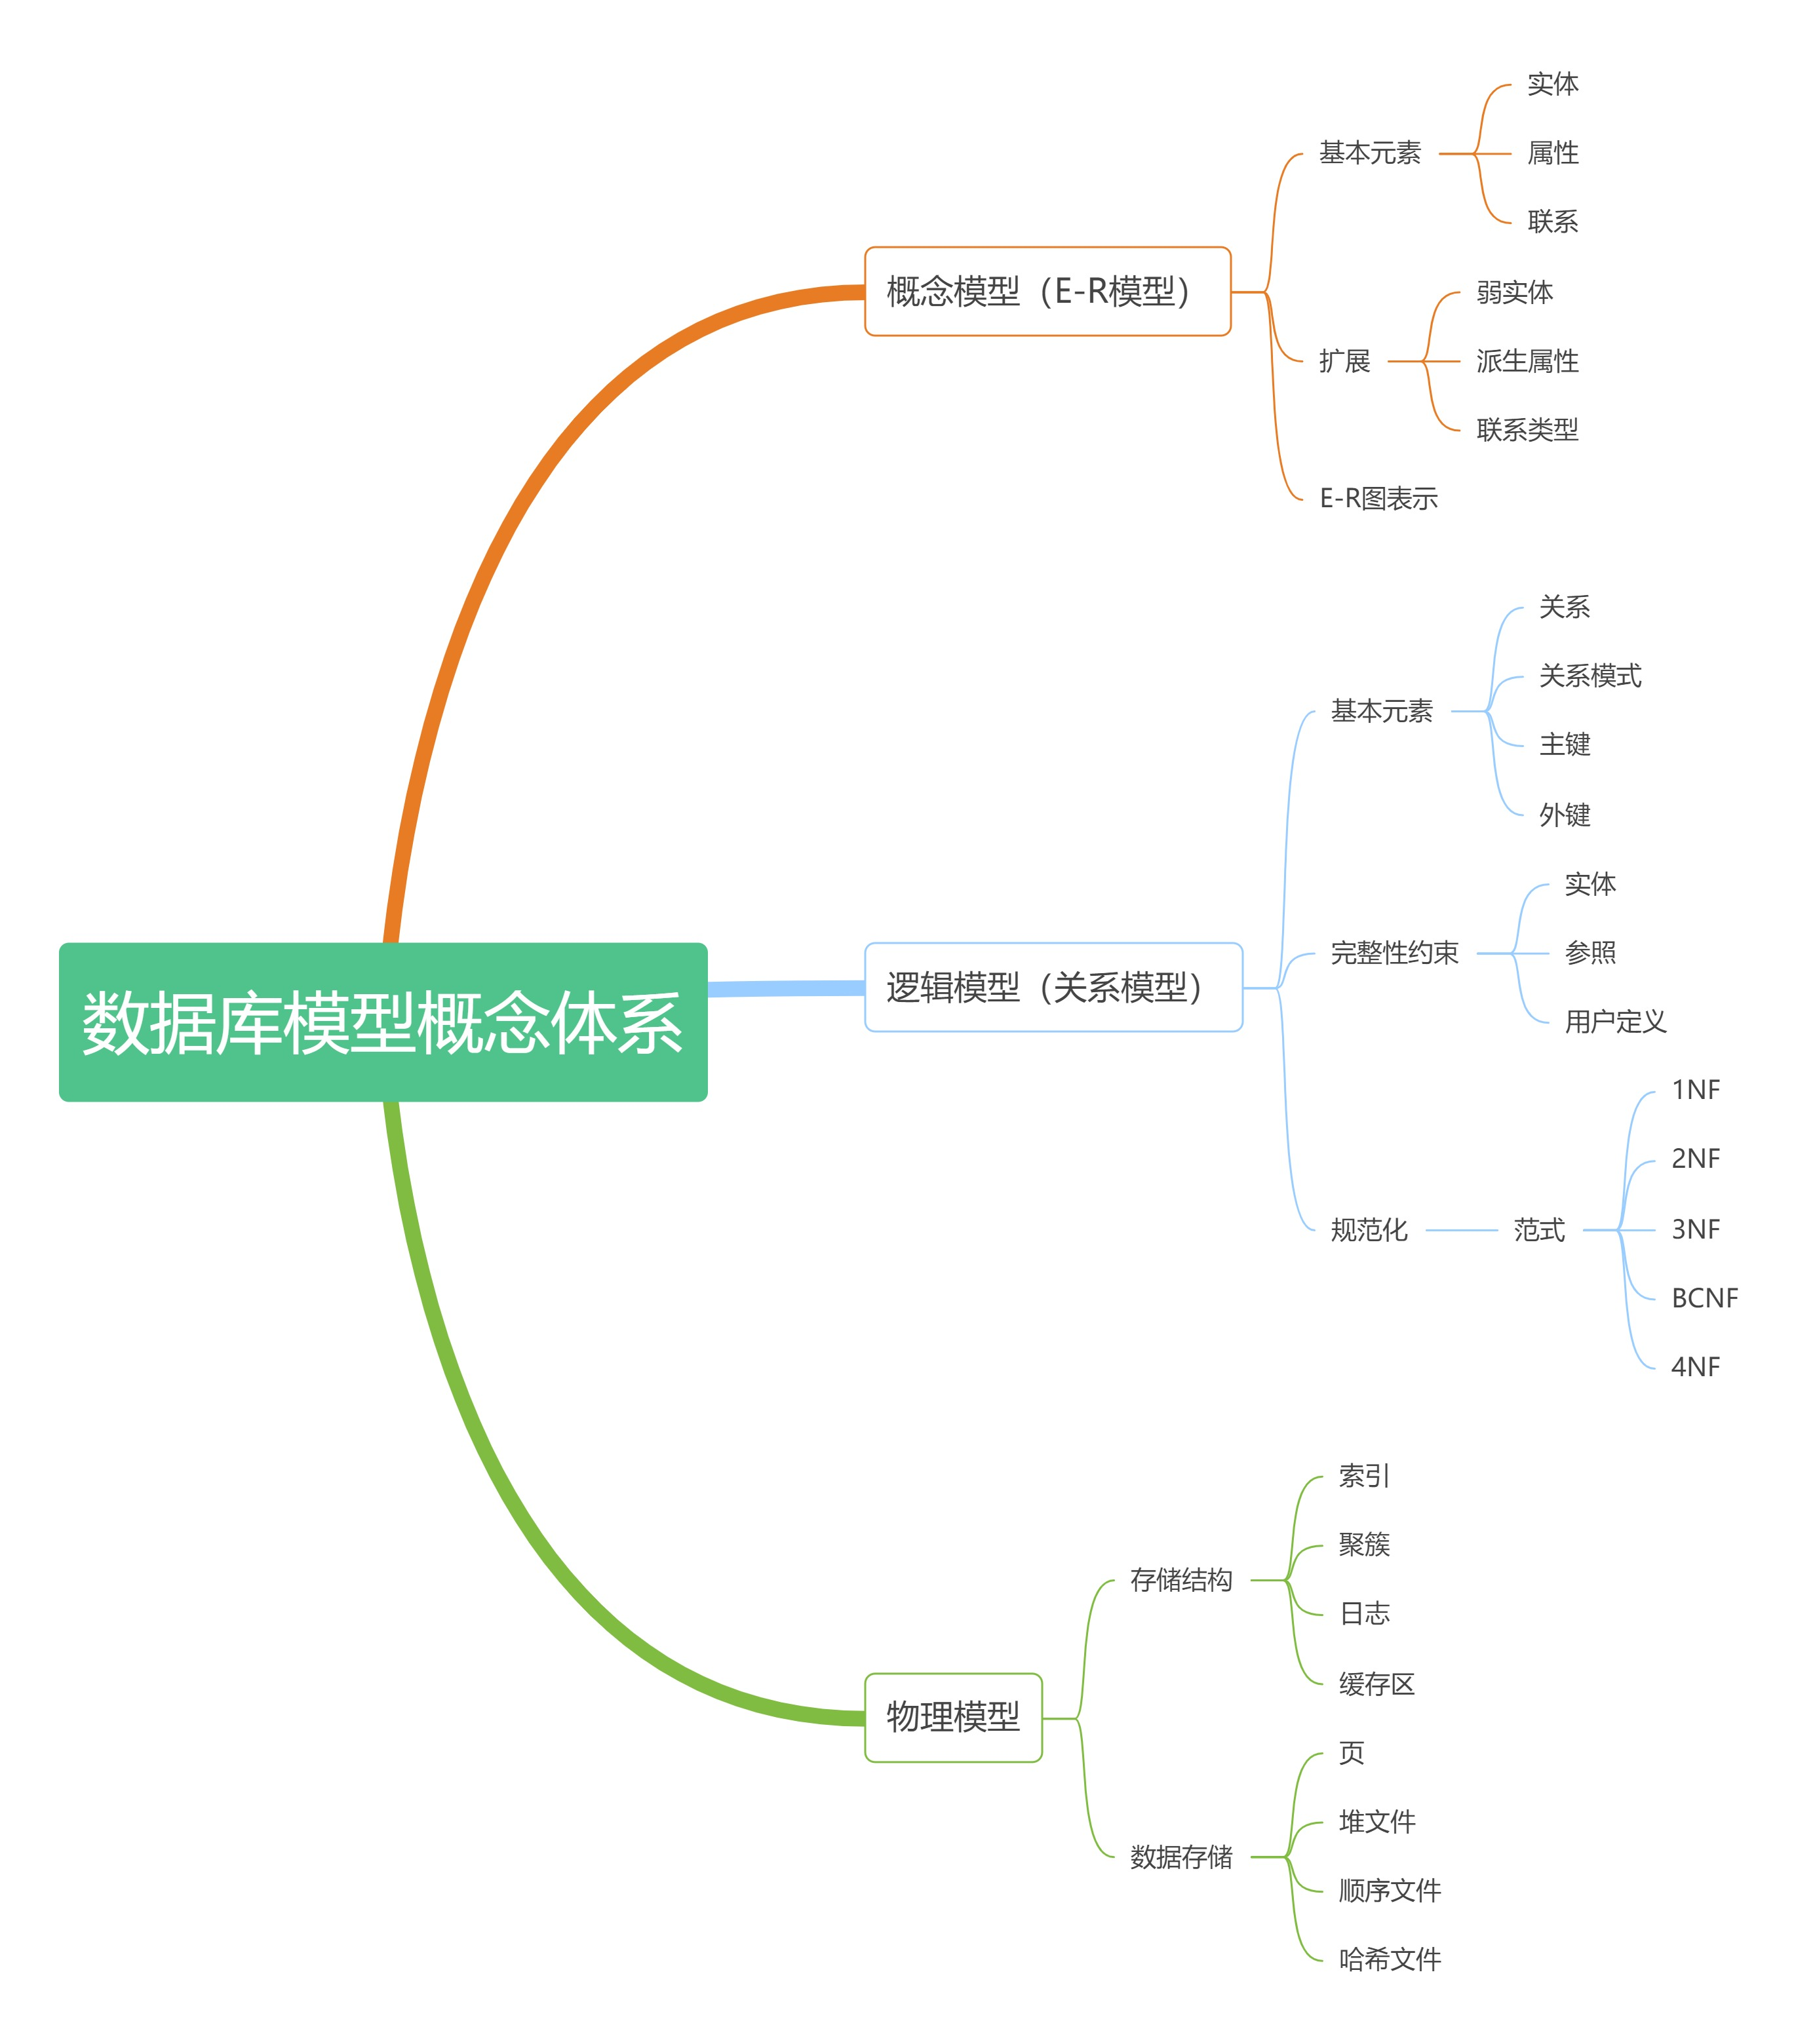
\includegraphics[width=0.8\textwidth]{static/images/数据库模型概念体系.jpg} % 调整宽度和路径
    \caption{数据库模型概念体系图} % 添加标题
    \label{fig:database-model-system} % 可选:添加标签以便引用
\end{figure}
\subsection{数据库设计阶段体系}
了解框架,如图\ref{fig:database-design}所示
可以看到,需求分析阶段和DFD挂钩,概念设计阶段和概念模型E-R图相关,逻辑设计和逻辑模型相关规范化,物理设计阶段和物理模型相关.
\FloatBarrier
\begin{figure}[H]
  \centering
  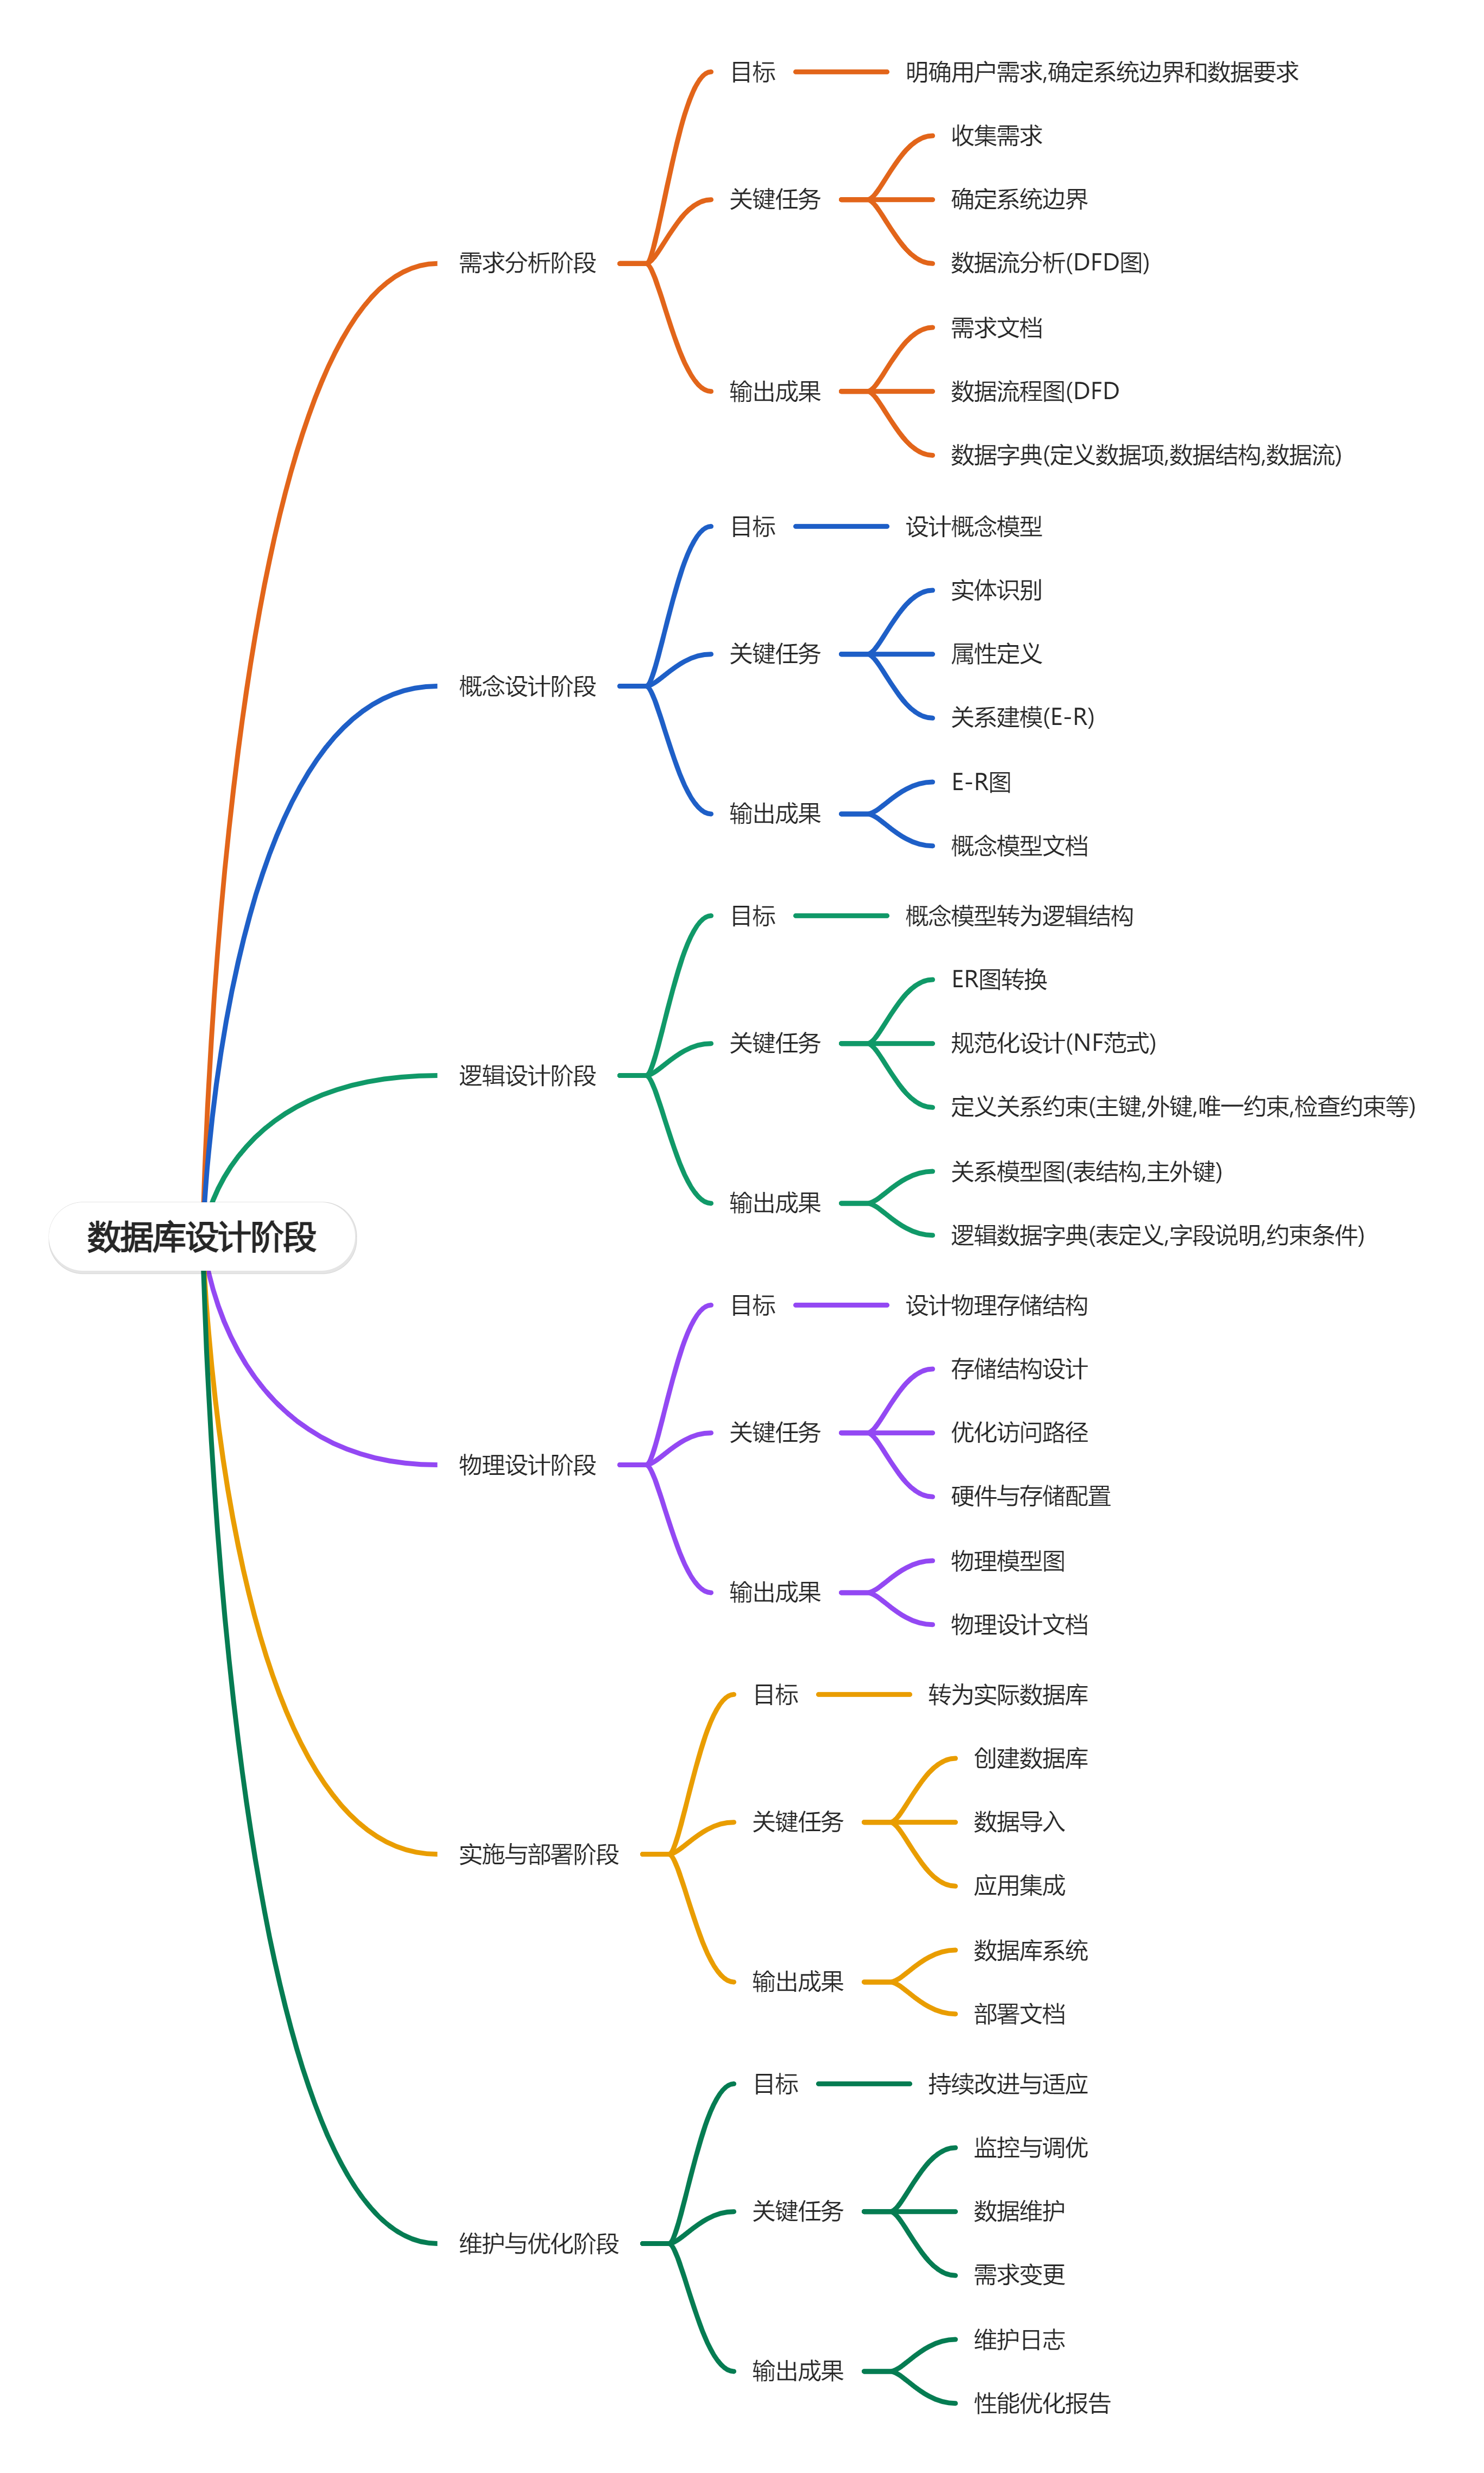
\includegraphics[width=0.8\textwidth]{static/images/数据库设计阶段图.png}
  \caption{数据库设计阶段图}
  \label{fig:database-design}
\end{figure}

\subsection{数据库三级模式}
主要注意哪些独立性和哪些模式相关,把握好对应关系,如图\ref{fig:database-three-level-mode}所示.
\FloatBarrier
\begin{figure}[H]
  \centering
  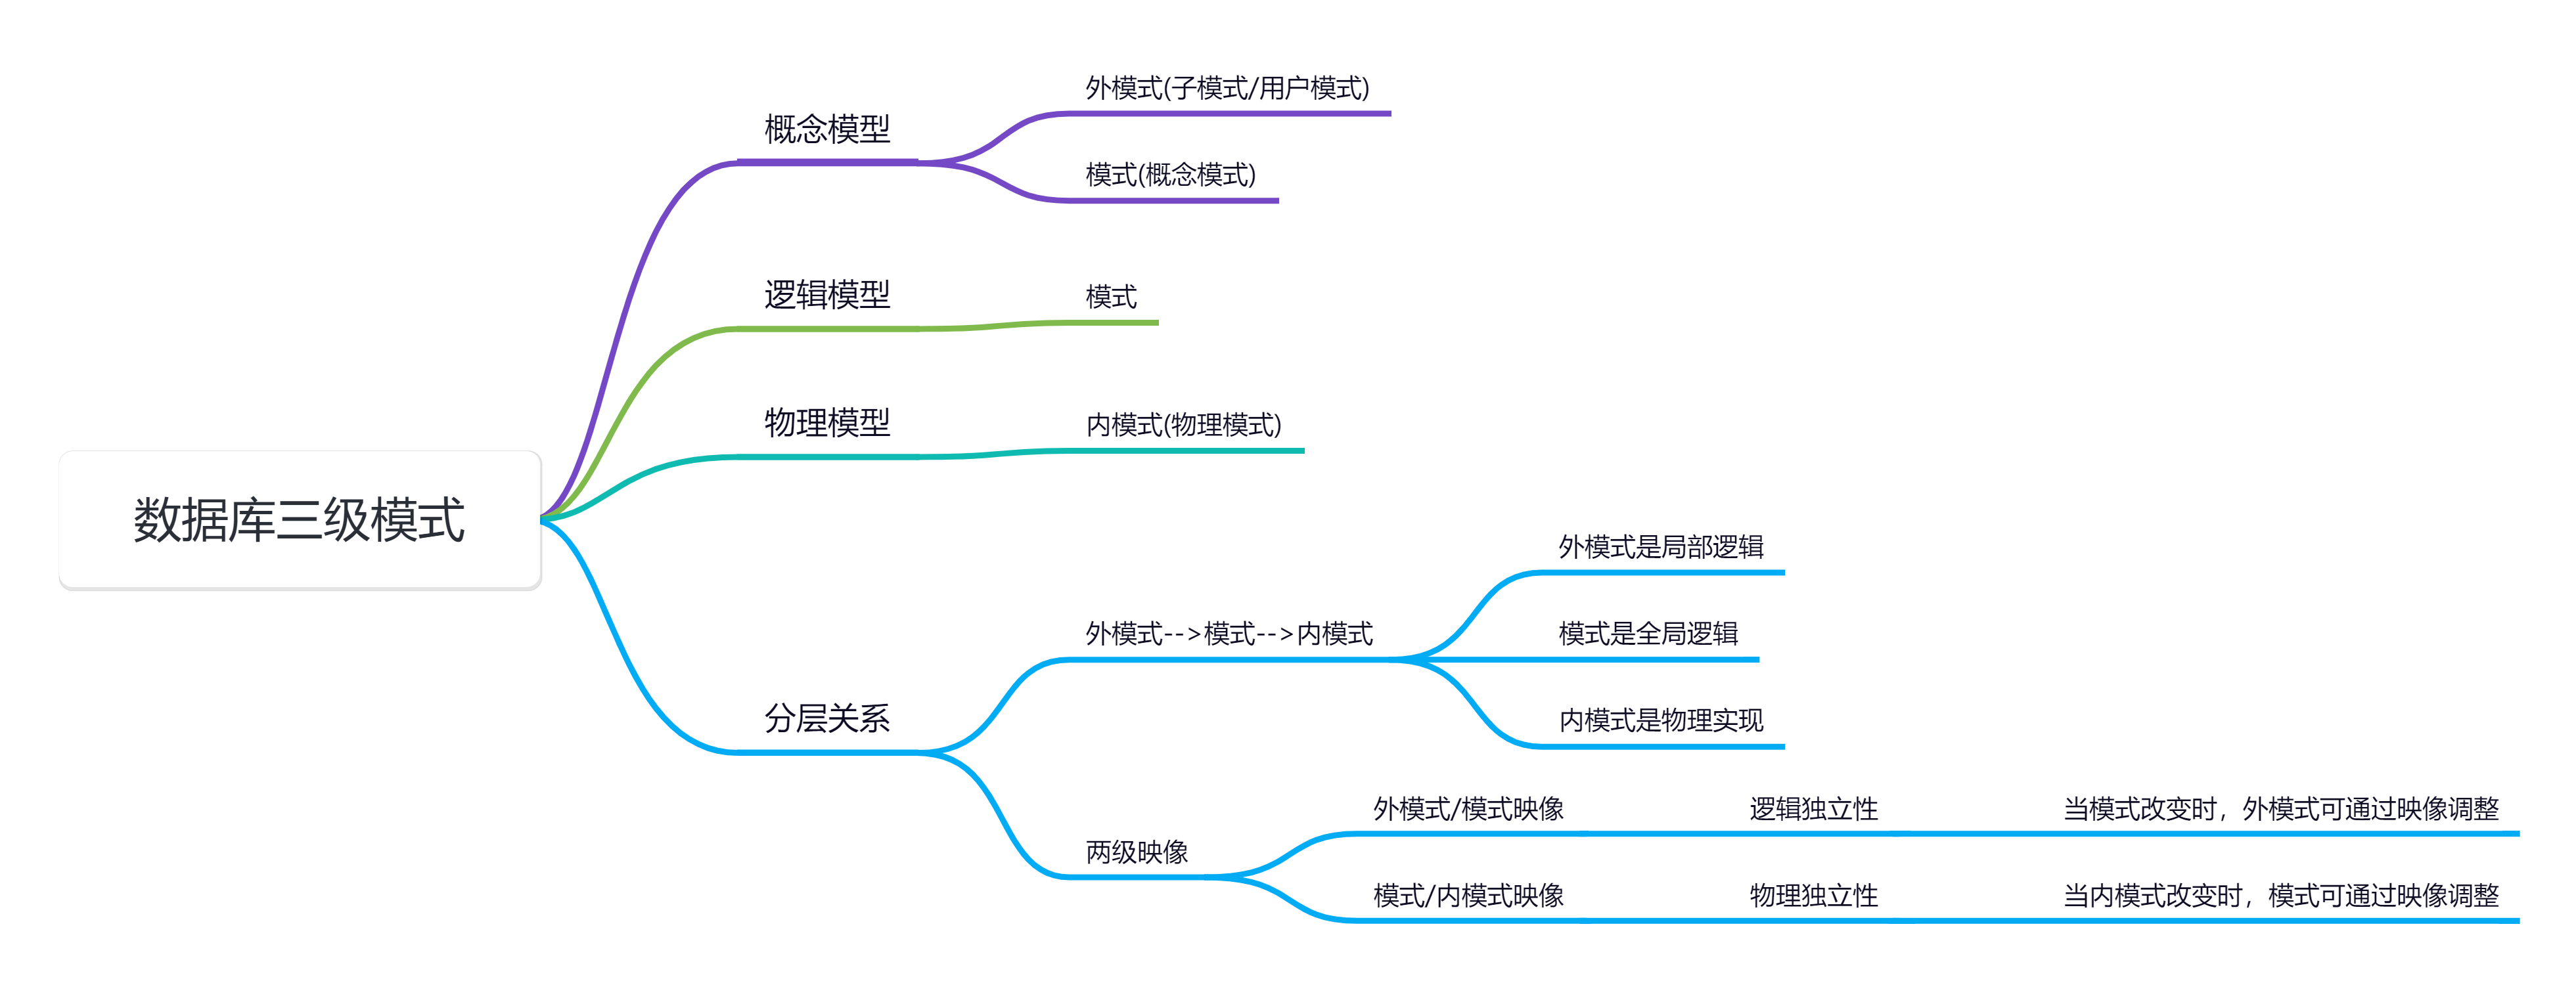
\includegraphics[width=0.8\textwidth]{static/images/数据库三级模式.png}
  \caption{数据库三级模式}
  \label{fig:database-three-level-mode}
\end{figure}
\subsection{小结}
选择填空常考的基础知识点,如图\ref{fig:database-base-knowledge}所示.
\FloatBarrier
\begin{figure}[H]
  \centering
  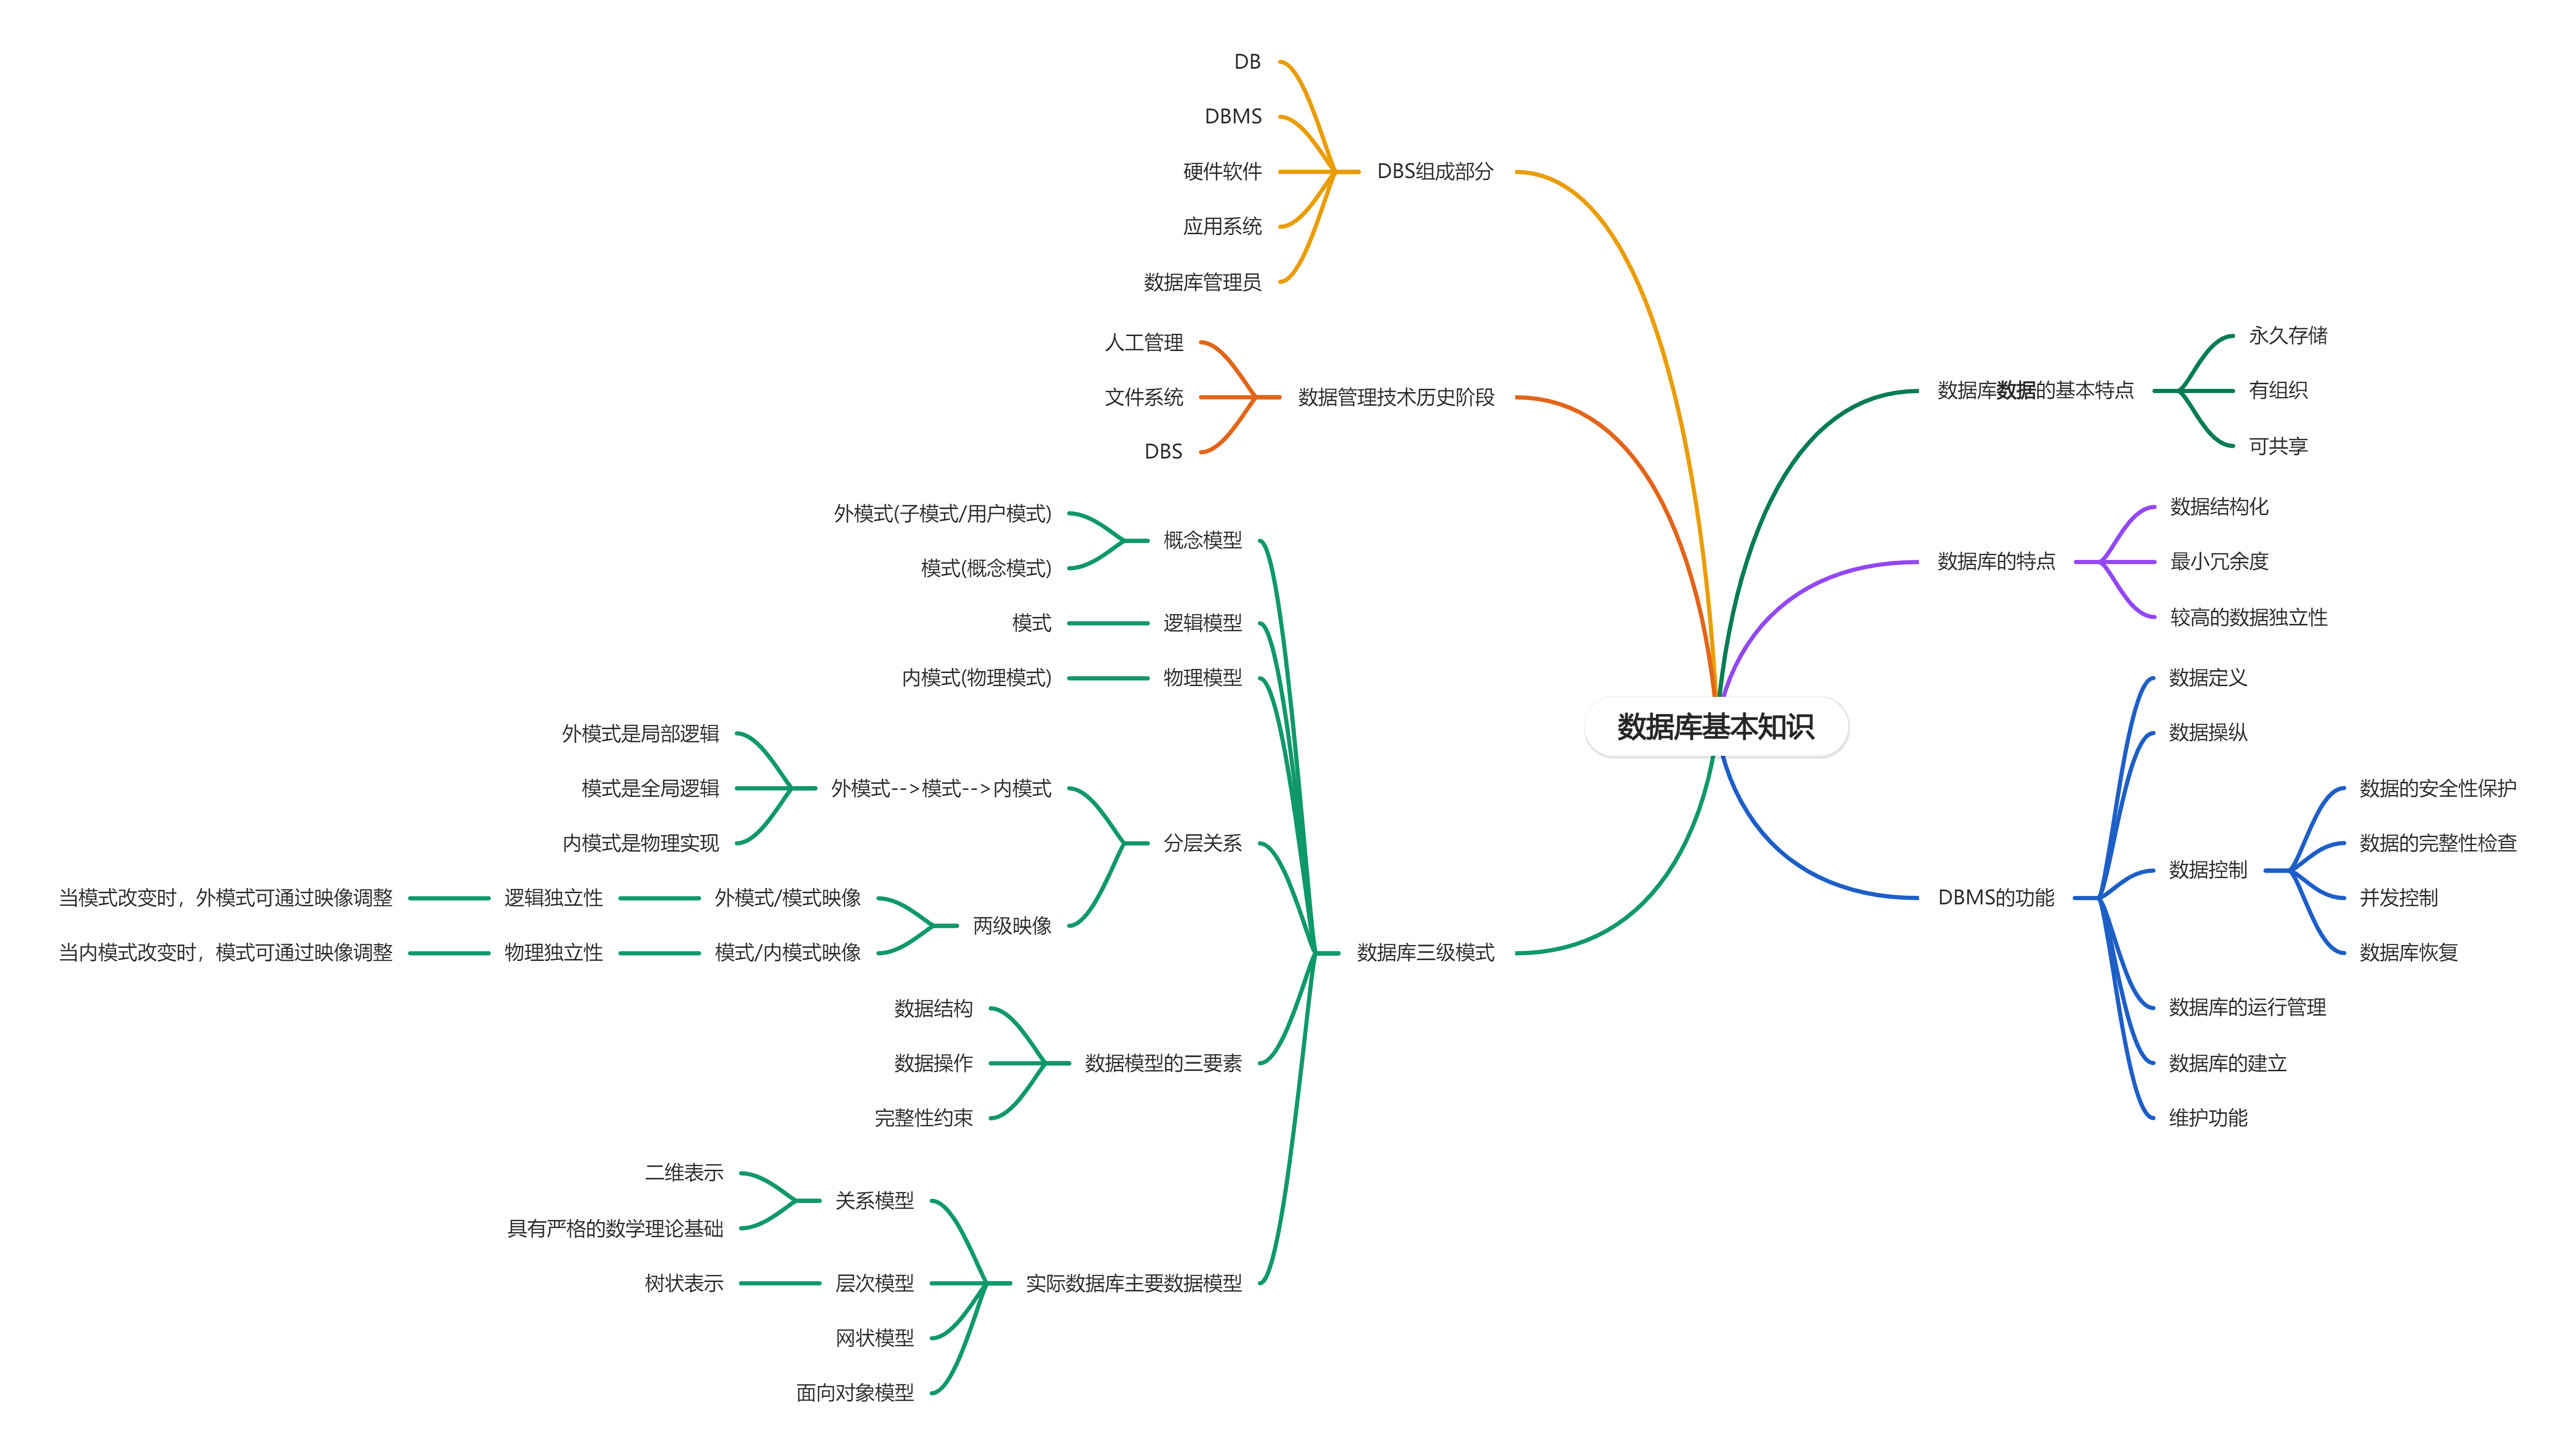
\includegraphics[width=0.8\textwidth]{static/images/数据库基本知识.png}
  \caption{数据库基本知识}
  \label{fig:database-base-knowledge}
\end{figure}
\newpage
\section{关系数据库}
\subsection{易混淆的概念}
\begin{enumerate}
  \item 关系代数是以\underline{集合运算}为基础的运算.
  \item 字段是列信息,记录是行信息,选择操作是对\textbf{\heiti 行/记录}操作,
  投影操作是对\textbf{\heiti 列/字段}操作.
  \item $R-S$表示在R但不在S的集合
\end{enumerate}
\subsection{常考填空}
如图\ref{fig:Relational-Database-Mind-Map} 所示,常见的分类和概念.
\begin{figure}[H]
  \centering
  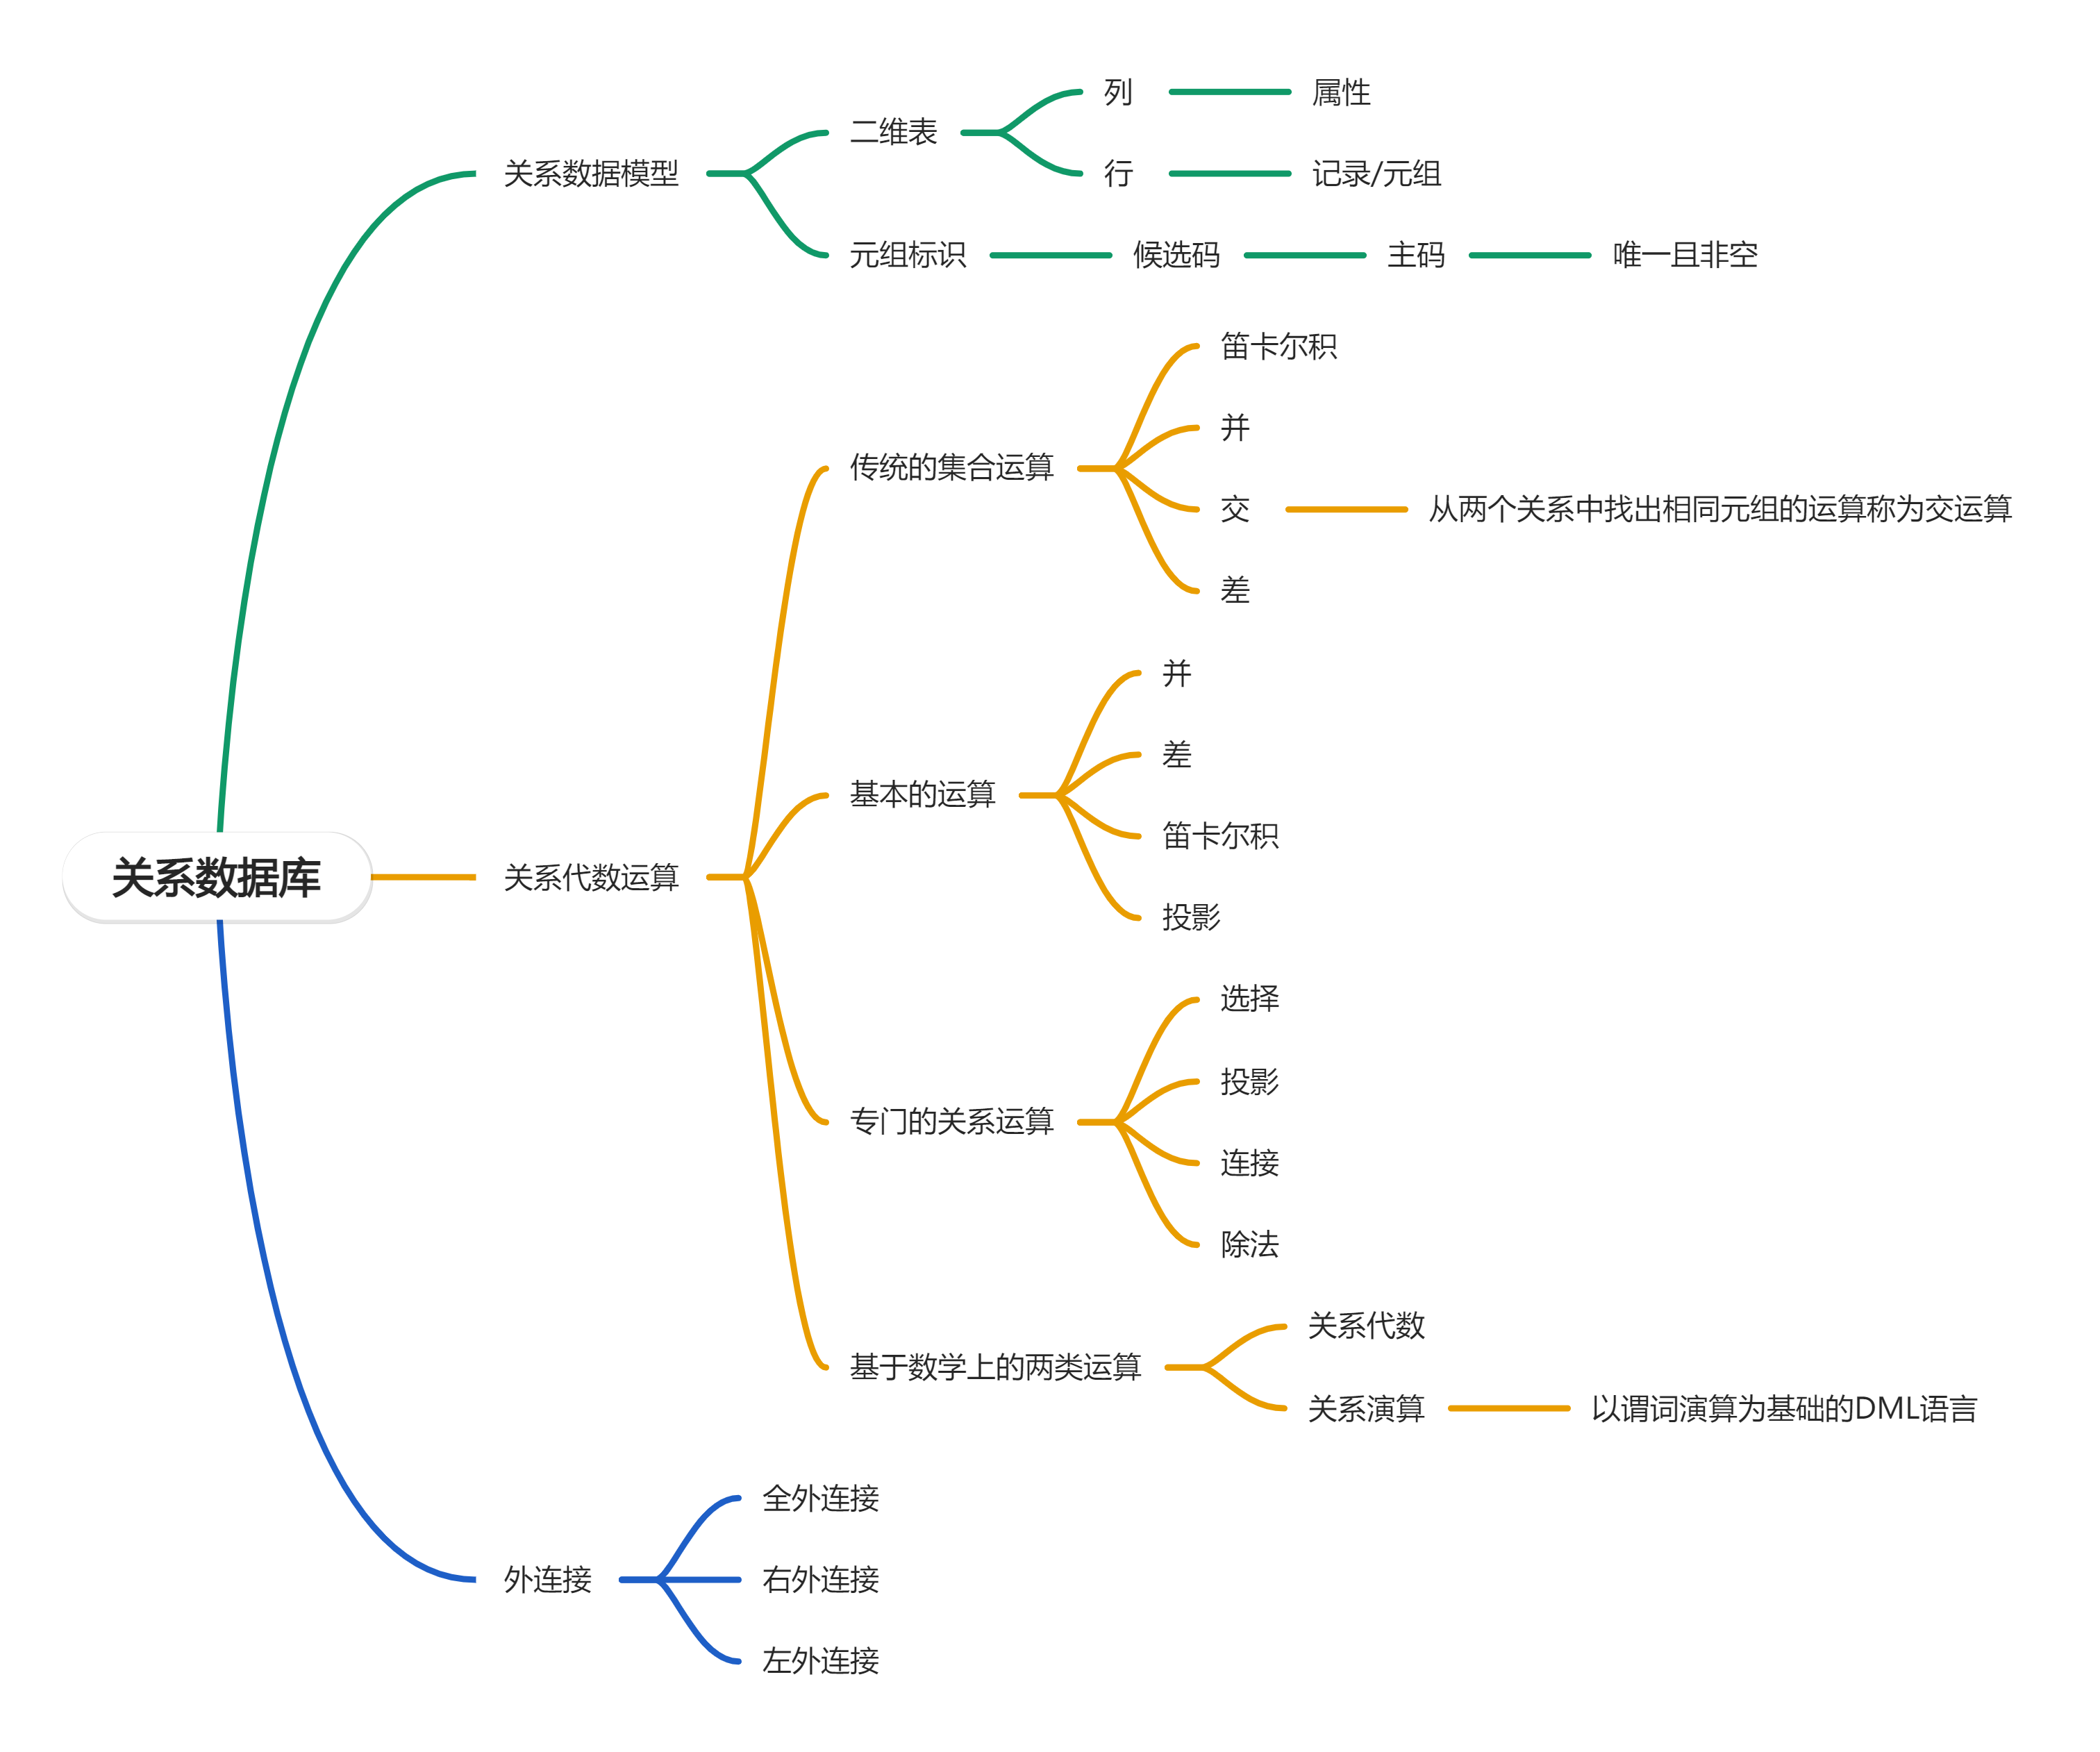
\includegraphics[width=0.8\textwidth]{static/images/关系数据库.png}
  \caption{关系数据库思维导图}
  \label{fig:Relational-Database-Mind-Map}
\end{figure}
\subsection{关系代数表达式例题}
\subsubsection*{eg. 在“学生一选课一课程”数据库中的3个关系如下:}

\begin{table}[H]
\centering
\caption{数据库中的3个关系}
\begin{tabular}{c c c c}
\toprule
S (S\#, SNAME, SEX, AGE) & SC (S\#, C\#, GRADE) & C (C\#, CNAME, TEACHER) \\
\midrule
\end{tabular}

\end{table}

查找选修“数据库技术”这门课程的学生的学生姓名和成绩,若用关系代数表达式来表示为:

\begin{equation*}%%\bowtie
\pi_{SNAME,GRADE} \big((S \bowtie SC )\bowtie (\sigma_{CNAME='\text{数据库技术}'} (C))\big) 
\end{equation*}
\newpage
\section{关系数据库标准语言SQL}
\subsection{错题知识点}
\begin{enumerate}
  \item 过程化
  注重流程,如何做
  \item 非过程化
  注重结果,做出什么
\end{enumerate}
删除行/记录是用:
\begin{lstlisting}
  DELETE row FROM TABLES
\end{lstlisting}
删除列/字段用:
\begin{lstlisting}
  ALTER TABLES DROP colomn
\end{lstlisting}
\subsection{常考填空}
\myitem SQL(Structured Query Language)的中文全称是\underline{结构化查询语言}
\myitem SQL功能:
\begin{itemize}
  \item 数据查询
  \item 数据定义
  \item 数据操纵
  \item 数据控制
\end{itemize}
\myitem \text{\heiti 基本表}有对应的物理存储,\text{\heiti 视图}没有对应的物理存储.
\par 视图是从\underline{基本表或视图}中导出的表,数据库中实际存放的是视图的\underbar{定义}.
\myitem DML(Data Manipulation Language)特点:
\begin{itemize}
  \item 操作对象与结果均为关系
  \item 操作的非过程性强
  \item 语言一体化
  \item 以数学理论为基础
\end{itemize}
\myitem 插入语句
\begin{lstlisting}
  INSERT INTO TABLES(field1,field2,field3,,,) VALUES(x,y,z,,,)
\end{lstlisting}
\myitem 修改语句
\begin{lstlisting}
  UPDATE TABLES SET field=vlaue 
  WHERE conditions
\end{lstlisting}
\myitem 删除语句
\begin{lstlisting}
  DELETE FROM TABLES 
  WHERE conditions
\end{lstlisting}
\myitem 例题
\subsubsection*{1. 设关系 R (A, B, C) 和 S (A, D, E, F),有 R.A=S.A。若将关系代数表达式:\(\pi_{R.A, R.B, S.D, S.F} (R \bowtie S)\) 用 SQL 语言的查询语句表示,则为:}
\par \begin{lstlisting}
SELECT R.A,R.B,S.D,S.F
FROM R,S
WHERE R.A=S.A
\end{lstlisting}
\subsubsection*{2. 在“学生一选课一课程”数据库中的3个关系如下:}

\begin{table}[h]
\centering
\caption{数据库中的3个关系}
\begin{tabular}{c c c c}
\toprule
S (S\#, SNAME, SEX, AGE) & SC (S\#, C\#, GRADE) & C (C\#, CNAME, TEACHER) \\
\midrule
\end{tabular}
\end{table}

查找选修“数据库技术”这门课程的学生的学生名和成绩。若使用连接查询的SQL语句是:
\par \begin{lstlisting}
  SELECT SNAME,GRADE
  FROM S
  JOIN SC ON S.S\#=SC.S\#
  JOIN C ON SC.C\#=C.C\#
  WHERE CNAME='数据库技术'
\end{lstlisting}

\subsubsection*{3.设有两个关系 R (A, B, C) 和 S (C, D, E),用 SQL 查询语句表达下列关系代数表达式 \(\pi_{A, E} (\sigma_{B=D} (R \bowtie S))\) 的语句是}
\par 答案:\begin{lstlisting}
  SELECT R.A,S.E FROM R
  JOIN S ON R.C=S.C
  WHERE R.B=S.D
\end{lstlisting}
\myitem 游标(Cursor)是数据库系统中用于逐行处理查询结果集的一种机制。
它允许应用程序对结果集中的数据执行精细控制,支持遍历、读取、更新或删除特定行,适用于需要逐行操作的场景。(类似于指针)
\begin{table}[H]
  \centering
  \caption{对比:游标 vs. 集合操作}
  \begin{tabular}{c c c}
  \toprule
  \textbf{特性} & \textbf{游标} & \textbf{集合操作} \\
  \midrule
  处理方式 & 逐行 & 批量 \\
  性能 & 低效 & 高效 \\
  适用场景 & 复杂逐行逻辑 & 简单查询、聚合、连接 \\
  资源占用 & 高 & 低 \\
  \bottomrule
  \end{tabular}
  \end{table}
  一个SQL语句原则上可产生或处理一组记录,而主语句一次只能处理一个记录,
  为此必须协调两种处理方式,这是通过使用\underline{游标或Cursor机制}来解决的。
\myitem DBMS中的语言系统分为\underline{主语言}和\underline{SQL语言}
\myitem \underline{删除/修改/插入操作}可以引发触发器.
\newpage
\section{数据库安全性}
\subsection{选择}
\subsubsection{安全性控制}
授权的数据对象的范围越小,授权子系统就越灵活;

授权的数据对象的约束越细致,授权子系统就越安全,但灵活性降低;
\subsection{填空}
\myitem 安全性问题包含\underline{技术安全类,管理安全类和政策法律类}
\myitem 鉴别用户的常用方法:\underline{用户名和口令}
\myitem 安全子系统由\underline{用户权限定义}和\underline{合法权检查机制}组成.
\myitem DBMS支持DAC(自主存取控制),有些还支持MAC(强制存取控制)
\begin{table}[htbp]
  \centering
  \caption{DAC和MAC对比总结}
  \begin{tabular}{p{3.5cm} >{\centering\arraybackslash}p{5cm} >{\centering\arraybackslash}p{5cm}}
  \toprule
  \textbf{对比项} & \textbf{DAC(自主访问控制)} & \textbf{MAC(强制访问控制)} \\
  \midrule
  主体与客体权限 & 用户自主决定 & 系统根据策略自动执行 \\
  灵活性 & 高(用户自主管理) & 低(系统策略决定) \\
  安全性 & 较低(可能出现权限传播问题) & 较高(严格控制权限) \\
  权限分配者 & 资源所有者 & 系统或管理员 \\
  常见应用场景 & 日常软件与常规数据库系统 & 军事、政府、机密系统 \\
  \bottomrule
  \end{tabular}
  \end{table}
\myitem 用户权限由\underbar{数据对象}和\underbar{操作类型}组成
\myitem 授权--GRANT;收回--REVOKE
\myitem 用户查看保护--视图机制
\myitem 审计分为\underbar{用户级}和\underbar{系统级}
\newpage
\section{数据库完整性}
\subsection{选择}
出现和\text{\heiti 主键}有关的完整性考点就选\textbf{\heiti 实体完整性}

出现和\text{\heiti 外键}有关的完整性考点就选\textbf{\heiti 参照完整性}

出现和\text{\heiti 自定义规则}有关的完整性考点就选\textbf{\heiti 用户定义的完整性}

\subsection{填空}
\myitem 数据库的完整性指的是数据的\underbar{正确性}和\underbar{相容性.}
\myitem 关系模型的完整性包括\underbar{实体完整性,参照完整性和用户定义完整性}.
\myitem 数据库完整性的定义一般由SQL的\underbar{DDL(Data Definition Language)}语句来实现,它们作为数据库模式的一部分存入\underbar{数据字典}中.
\myitem 实体完整性在\underbar{CREATE TABLE}中用\underbar{PRIMARY KEY}定义.
\myitem 参照完整性在\underbar{CREATE TABLE}中用\underbar{FOREIGN KEY}定义外码,用\underbar{REFERENCE}指明这些外码参照哪些表的主码.
\par 延伸扩展,如图\ref{fig:SQL-Language-Classification}所示,SQL语言分类
\begin{figure}[H]
  \centering
  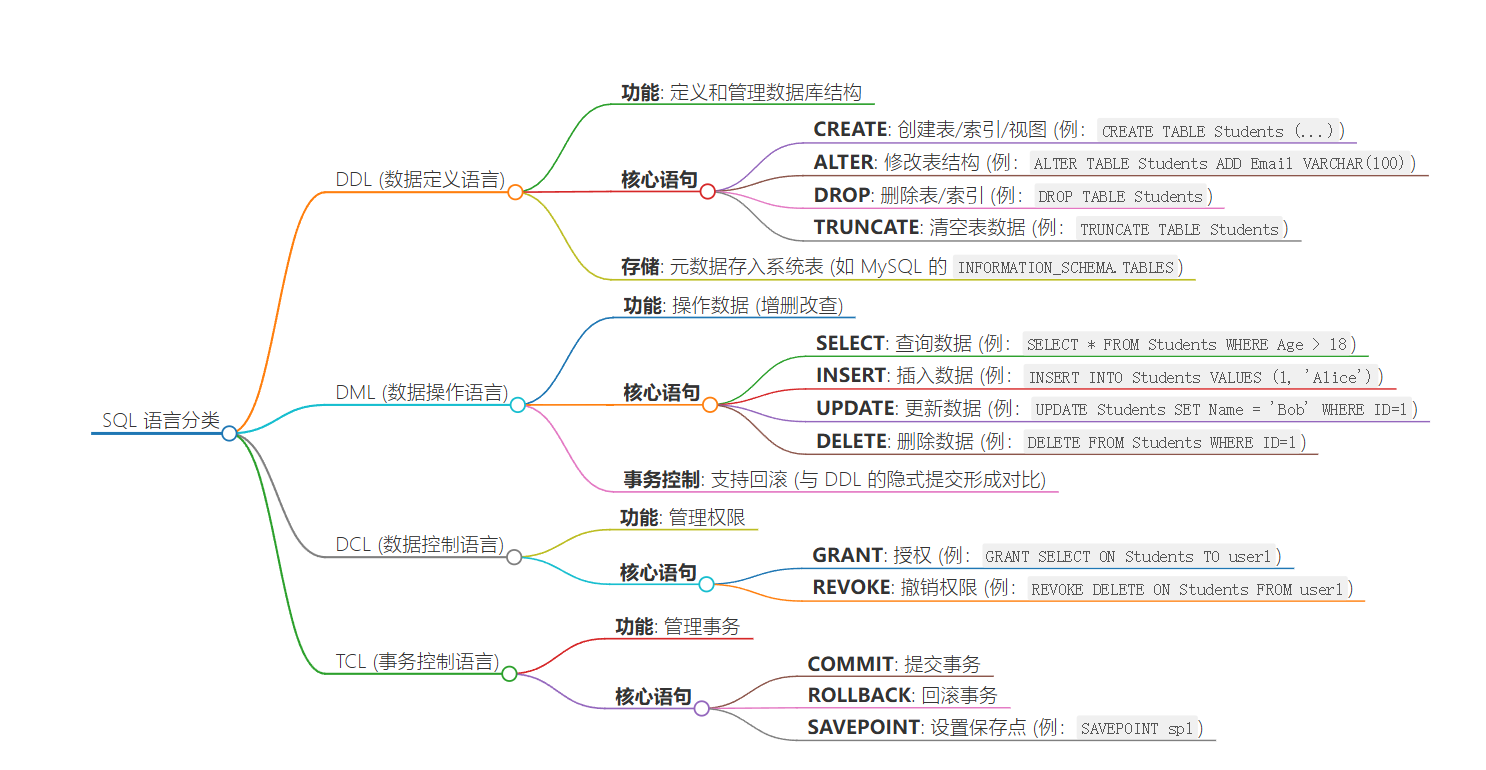
\includegraphics[width=0.8\textwidth]{static/images/SQL语言分类.png}
  \caption{SQL语言分类图}
  \label{fig:SQL-Language-Classification}
\end{figure}
\newpage
\section{关系数据理论}
\subsection{选择}
规范化,如表\ref{tab:normal-forms}所示
\begin{table}[H]
  \centering
  \caption{数据库范式核心条件}
  \label{tab:normal-forms}
  \begin{tabularx}{\textwidth}{@{}lX@{}} % 使用tabularx环境,自动填满文本宽度
  \toprule
  \textbf{范式} & \textbf{定义与核心条件} \\
  \midrule
  1NF (原子范式) & 所有属性值为不可再分的原子值,但存在非主属性对候选键的\textbf{部分函数依赖}。 \\
  2NF (候选键范式) & 满足1NF,且非主属性完全函数依赖于候选键,但存在非主属性对候选键的\textbf{传递函数依赖}。 \\
  3NF (第三范式) & 满足2NF,且不存在传递函数依赖,但允许非主属性之间存在依赖关系。 \\
  BCNF (巴斯-科德范式) & 满足3NF,且所有函数依赖的决定因素均为\textbf{超键}(候选键或主键)。 \\
  4NF (第四范式) & 满足BCNF,且不存在非平凡的\textbf{多值依赖}(即属性间无非平凡的多值关联)。 \\
  5NF (第五范式/投影-连接范式) & 满足4NF,且不存在非平凡的\textbf{连接依赖},确保关系无法通过投影-连接分解为更小的关系集合。 \\
  \bottomrule
  \end{tabularx}
\end{table}
\subsection{填空}
\myitem 合并规则:$X\rightarrow Y$ 和 $Y\rightarrow Z$ 时,可以推导出 $X \rightarrow YZ$.
\myitem 平凡函数依赖可以通过自反律推出
\begin{itemize}
  \item 平凡函数依赖:$Y \subseteq X \Rightarrow X \rightarrow Y$ 总成立,信息量小。
  \item 自反律:$X \rightarrow X$ 总成立,是平凡依赖的特例(当 $Y = X$ 时)。
\end{itemize}
\myitem 规范化设计中,对模式等价分解时,要具有\underline{无损连接性}和\underline{保持函数依赖}.
\myitem 多种数据依赖,其中最重要的是\underbar{函数依赖}和\underbar{多值依赖}.
\myitem 设关系模式 R (A,B,C),F 是 R 上成立的 FD 集,F = \{B→A,B→C\},则分解 ρ  = \{AB,AC\}丢失的 FD 是 ?。
\par 易知,候选键为B,其中B->A,B->C,但在AB中不包含C,AC中不包含B,即B->C不成立,所以丢失$B \rightarrow C$.
\myitem 关系范式不属于2NF时,会产生\underline{插入异常,删除异常和修改复杂},只满足1NF的关系可能存在\text{\heiti 数据冗余大,修改异常,插入异常和删除异常}.
\myitem 两个函数依赖集等价的充要条件为\underbar{F包含在G的超集,G包含在F的超集中}.
\newpage
\section{数据库设计}
\myitem 数据库建设的基本规律:"三分技术,七分管理,十二分基础数据".
\myitem 规范设计法的基本思想是\underbar{过程迭代}和\underbar{逐步求精}.
\myitem 数据库的生命周期可分为两个阶段,一是\underbar{数据库需求分析和设计阶段},二是\underbar{数据库实现和运行阶段}.
\myitem 数据库设计阶段可分为:\underbar{需求分析,概念结构设计,逻辑结构设计,物理设计阶段,数据库实施阶段,数据库运行和维护阶段}.
\myitem 数据库实施阶段包括\underbar{组织数据入库}和\underbar{应用程序的编码和测试}.
\myitem 数据库的物理设计分为两步,一是确定数据库的\underbar{物理结构},二是对其评价,指标为\underline{空间}和\underline{时间效率}.
\par 具体设计阶段如图\ref{fig:Database-design-phase}所示
\begin{figure}[H]
  \centering
  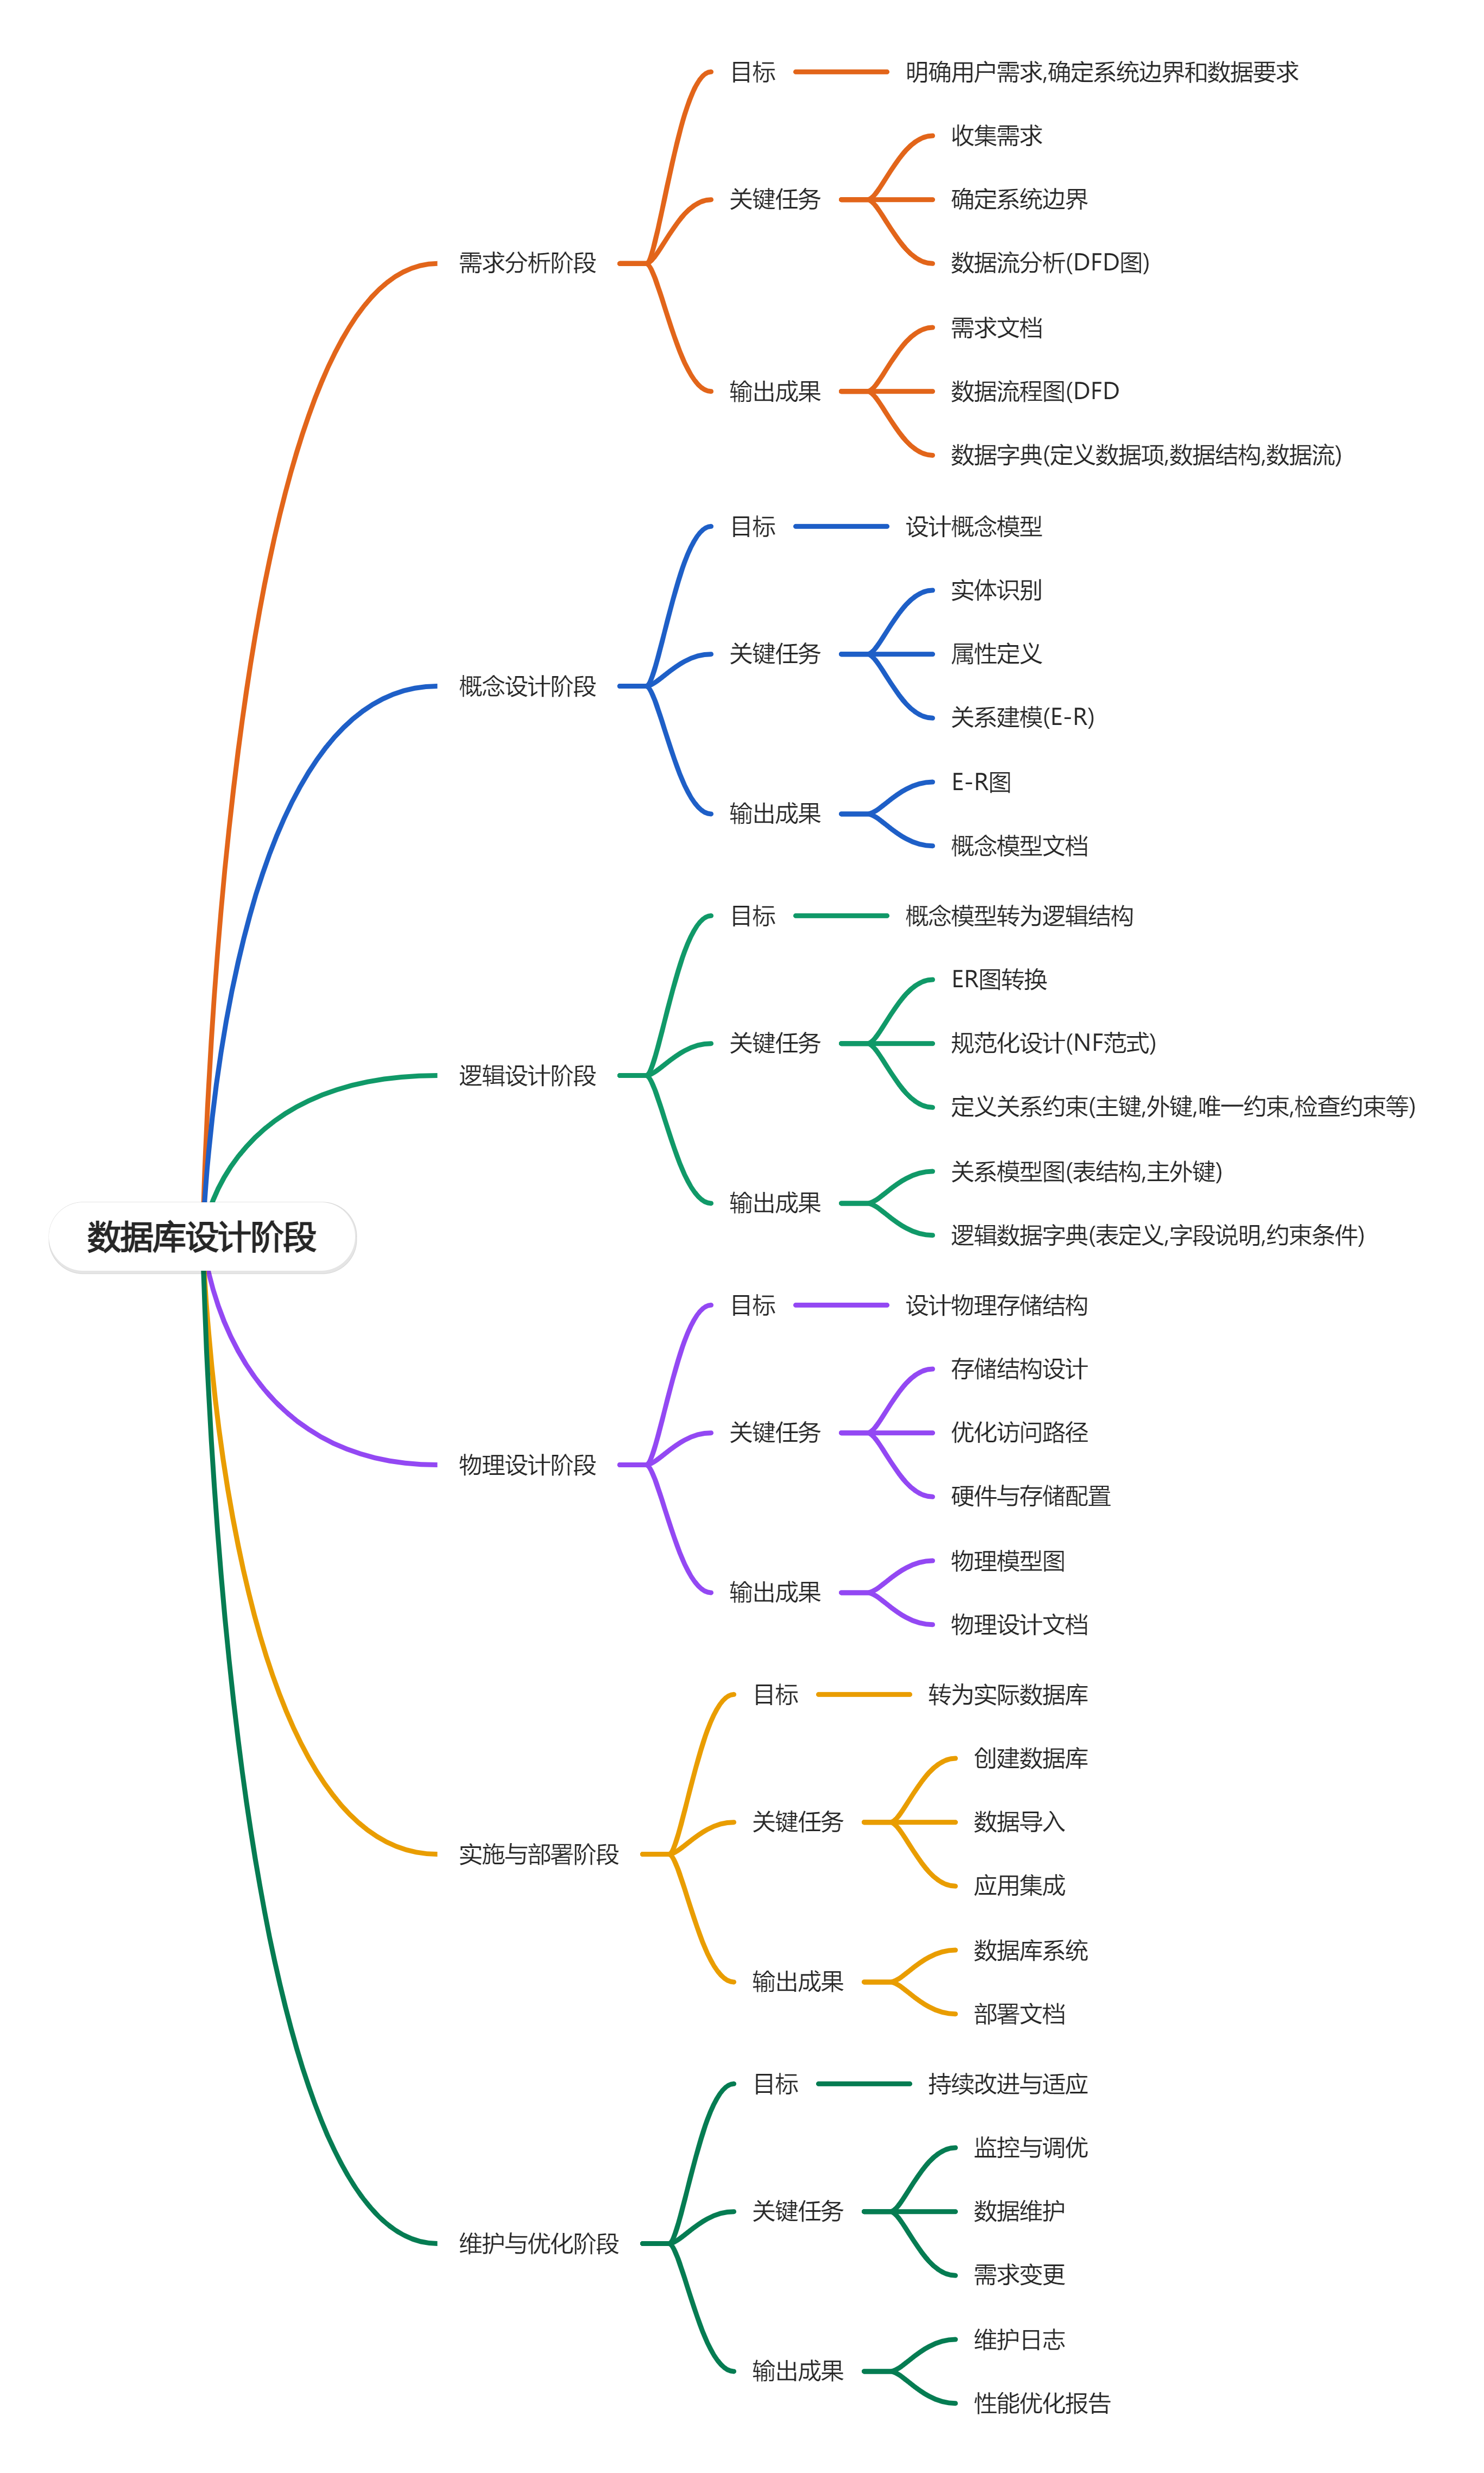
\includegraphics[width=0.6\linewidth, keepaspectratio]{static/images/数据库设计阶段图.png}
  \caption{数据库设计阶段图}
  \label{fig:Database-design-phase}
\end{figure}
\myitem 按应用目的分类,模型可分为\underbar{概念模型}和\underbar{数据模型}.
\myitem 类的继承提高了软件的\underbar{可重用性/共享性},继承的模型称为\underline{子模型}.
\myitem 概念结构是对现实世界中的一种抽象,抽象有\underline{分类,聚集,概括}.
\myitem E-R图设计冲突主要来自\underline{属性,命名和结构}.
\newpage
\section{数据库恢复技术}
\subsection{易错概念}
\myitem 事务的持续性是永久的,一旦提交,对数据库的改变是永久的.
\myitem 事务日志用于保存\underbar{关于"数据"和"更新数据"}相关的操作(必须是数据,且数据要发生改变).
\subsection{填空}
\myitem 数据库应用程序的基本逻辑单元是\underline{事务}.
\myitem 事务处理技术主要包括\underline{数据库恢复技术}和\underbar{并发控制技术}.
\myitem 事务的特性:\underline{原子性(Atomicity),一致性(Consistency),隔离性(Isolation),持续性(Durability)},也称为\textbf{ACID}
\myitem 数据库系统故障分为:\underline{事务故障,系统故障,介质故障,计算机病毒}.
\myitem 建立冗余数据最常用的技术是\underline{数据转储}和\underline{登录日志文件}
\myitem 转储可分为\underline{静态转储}和\underline{动态转储},转储方式可分为\underline{海量转储}和\underline{增量转储}.
\myitem \text{\heiti 日志文件}是用来记录事务对数据的更新操作的文件.\quad 主要分为两种格式:以\underline{记录}为单位和以\underline{数据块}为单位的日志文件.
\newpage 
\section{并发控制}
\myitem 死锁是\text{\heiti 资源分配策略不当}导致的,两个或多个事务同时处于互相等待状态,称为死装.
\myitem 并发操作带来的问题包括:\underline{读取"脏"数据,丢失修改,不可重复读}
\myitem 多个事务的并发执行是正确的,当且仅当其结果与按某一次序串行地执行它们的结果相同,我们称这种调度策略为\underbar{可串行化}的调度。
\myitem \text{\heiti 封锁对象的大小}被称为封锁的颗粒度.
\myitem 封锁类型分为\underline{排他锁(Exclusive Locks)--X锁}和\underline{共享锁(Share Locks)--S锁}.(巧记:首字母大小,E不发音)


\end{document}